\documentclass[10pt,a4paper]{article}
\usepackage[latin1]{inputenc}
\usepackage{amsmath}
\usepackage{amsfonts}
\usepackage{amssymb}
\usepackage{float}
\usepackage{graphicx}
%\usepackage{combine}
\begin{document}
\title{Design of experiment - exploring the boiling time of water with different parameters}
\author{Espen J. Velsvik and Anders O. Voldsund}
\maketitle

\section{Introduction}
In a world where the electric kettles are in a dominant position for heating water for your daily afternoon tea, the amount of people using cooking pots are dropping, with good reason. The superiority of the electric kettles when it comes to time usage, is well established.

If you are one of those that still use a cooking pot for heating water, we aim to give you the answers for what can be done about the problem. Don't be one of those people wasting time heating water when you instead could have taken dance lessons or learned a new language. Sure it won't be the same as electric kettles, but still, time is valuable in today's society.

Although a lot of people heat the water without a lid, it is known that it heats faster with one. We think this will indeed affect the results. Besides that we feel there are few established "myths" when it comes to what affects the time for boiling water.

In this project we want to study how different parameters affects the boiling time of water when using a cooking pot. If we can figure out the best way of boiling water efficiently, we finally have time to complete the great works of Henrik Ibsen that we have been longing to do.

\section{Selection of factors and levels}
\begin{table}[H] \centering 
  \caption{Factors used in the experiment} 
  \label{factors} 
\begin{tabular}{@{\extracolsep{5pt}} cccccc} 
\\[-1.8ex]\hline 
\hline \\[-1.8ex] 
 & A & B & C & D &\\ 
1 & Lid & Large pot & Soap & Olive oil \\ 
-1 & Without lid & Small pot & No soap & No olive oil\\ 
\hline \\[-1.8ex] 
\end{tabular} 
\end{table} 

We have chosen four factors that we think will be relevant to the problem. Notice that the size of the cooking plate is not the same for the pot sizes. The large pot was set on a large cooking plate, while the small pot was on a small cooking plate.

We had a hope that factor $C$ and $D$ would affect the boiling time individually, but also that the interaction between them would be significant. As olive oil is non polar, it doesn't mix with water. It will, however, mix if the soap is added. We suspected that the olive oil would increase the boiling time because it would affect the surface tension of the water, and maybe make it harder for the water to evaporate, hence delay the boiling state.

The two last factors had a level where low was without anything, while the high level was with two spoons of the substance, about 30 mL.

In this experiment it is easy to control if the factors are at the desired level, because we see if the lid is on, how large the pot is, and if the soap or the olive oil have been added.

\section{Selection of response variable}
In our problem we have chosen the time measured in seconds from cold water to boiling water. The choice of response variable could, in retrospect, have been chosen better. This is because it is hard to know exactly when the boiling state occurs. Because we were two people performing the experiments, and we had slightly different standards for when it was boiling, the accuracy of the measurements was reduced.

Another possible variable could be measuring the temperature of the water, and determine the time taken to achieve that temperature. From \cite{teaTemperatures} we know that the green teas have delicate leaves, and thus the water temperature must be between $77 ^\circ$C and $85 ^\circ$C. As green teas are our cup of tea, a temperature of about $80 ^\circ$C could be a temperature where we would stop the time. This way we will not cook the leaves and ruin their delicate flavors. Apart from the olive oil and the soap, obviously, which is a minor issue. If you on the other hand have a real craving for some herbal tea, a temperature of $98 ^\circ$C will do the trick.

\section{Choice of design}
A $2^k$ factorial design was conducted. As we had 4 factors, we did 16 experiments. The table shows the different combinations.

\begin{table}[H] \centering 
  \caption{DOE: $2^k$ full factorials} 
  \label{DOEtable} 
\begin{tabular}{@{\extracolsep{5pt}} cccccc} 
\\[-1.8ex]\hline 
\hline \\[-1.8ex] 
 & A & B & C & D & y \\ 
1 & -1 & -1 & -1 & -1 & $195$ \\ 
2 & 1 & -1 & -1 & -1 & $168$ \\ 
3 & -1 & 1 & -1 & -1 & $85$ \\ 
4 & 1 & 1 & -1 & -1 & $86$ \\ 
5 & -1 & -1 & 1 & -1 & $169$ \\ 
6 & 1 & -1 & 1 & -1 & $210$ \\ 
7 & -1 & 1 & 1 & -1 & $101$ \\ 
8 & 1 & 1 & 1 & -1 & $97$ \\ 
9 & -1 & -1 & -1 & 1 & $172$ \\ 
10 & 1 & -1 & -1 & 1 & $177$ \\ 
11 & -1 & 1 & -1 & 1 & $94$ \\ 
12 & 1 & 1 & -1 & 1 & $100$ \\ 
13 & -1 & -1 & 1 & 1 & $224$ \\ 
14 & 1 & -1 & 1 & 1 & $213$ \\ 
15 & -1 & 1 & 1 & 1 & $93$ \\
16 & 1 & 1 & 1 & 1 & $73$ \\
\hline \\[-1.8ex] 
\end{tabular} 
\end{table} 

\section{Implementation of the experiment}
Before we did the experiment we calculated 16 random numbers on a webpage, and we did it in that sequence. This would have worked fine if it wasn't for the lack of uniqueness of the numbers. After having done experiment 3 four times, we sensed something was wrong. Because we were two persons, we could do two experiments at the same time. A little slack was introduced, as we managed to get six experiments in a row using only the small pot.

Not doing the experiments in a specific order is called randomization, i.e. the run order is random. The reason for this is that potential external factors are not confounded with experimental factors.  We also focused on doing genuine run replicates. This means that all external factors should be equal for every experiment, at least the ones we can control. I.e. for every experiment the pot was cooled in cold water, and the lid as well. Afterwards the pots were dried. To get equal temperatures on the cooking plates, the temperature was set to maximum the entire time. In every experiment we used the same amount of water, 2.5 dL.

\section{Analysis of data}
In table \ref{effects1} and table \ref{effects2}, you can see the main effects and the interaction effects. As one can see, the effect of $B$ is a lot larger than the other effects. 

\begin{table}[H] \centering 
  \caption{Effects} 
  \label{effects1} 
\begin{tabular}{@{\extracolsep{5pt}} cccccccc} 
\\[-1.8ex]\hline 
\hline \\[-1.8ex] 
(Intercept) & A1 & B1 & C1 & D1 & A1:B1 & A1:C1 & A1:D1\\ 
$282.125$ & $$-$1.125$ & $$-$99.875$ & $12.875$ & $4.375$ & $$-$3.125$ & $2.625$ & $$-$3.875$\\ 
\hline \\[-1.8ex] 
\end{tabular} 
\end{table}

\begin{table}[H] \centering 
  \caption{Effects} 
  \label{effects2} 
\begin{tabular}{@{\extracolsep{5pt}} cccccccc} 
\\[-1.8ex]\hline 
B1:C1 & B1:D1 & C1:D1 & A1:B1:C1 & A1:B1:D1 & A1:C1:D1 & B1:C1:D1 & A1:B1:C1:D1\\ 
-13.125 & -6.625 & 2.125 & -10.375 & 1.125 & -13.125 & -15.875 & 7.875\\ 
\hline \\[-1.8ex] 
\end{tabular} 
\end{table}


\begin{figure}[p]
    \centering
    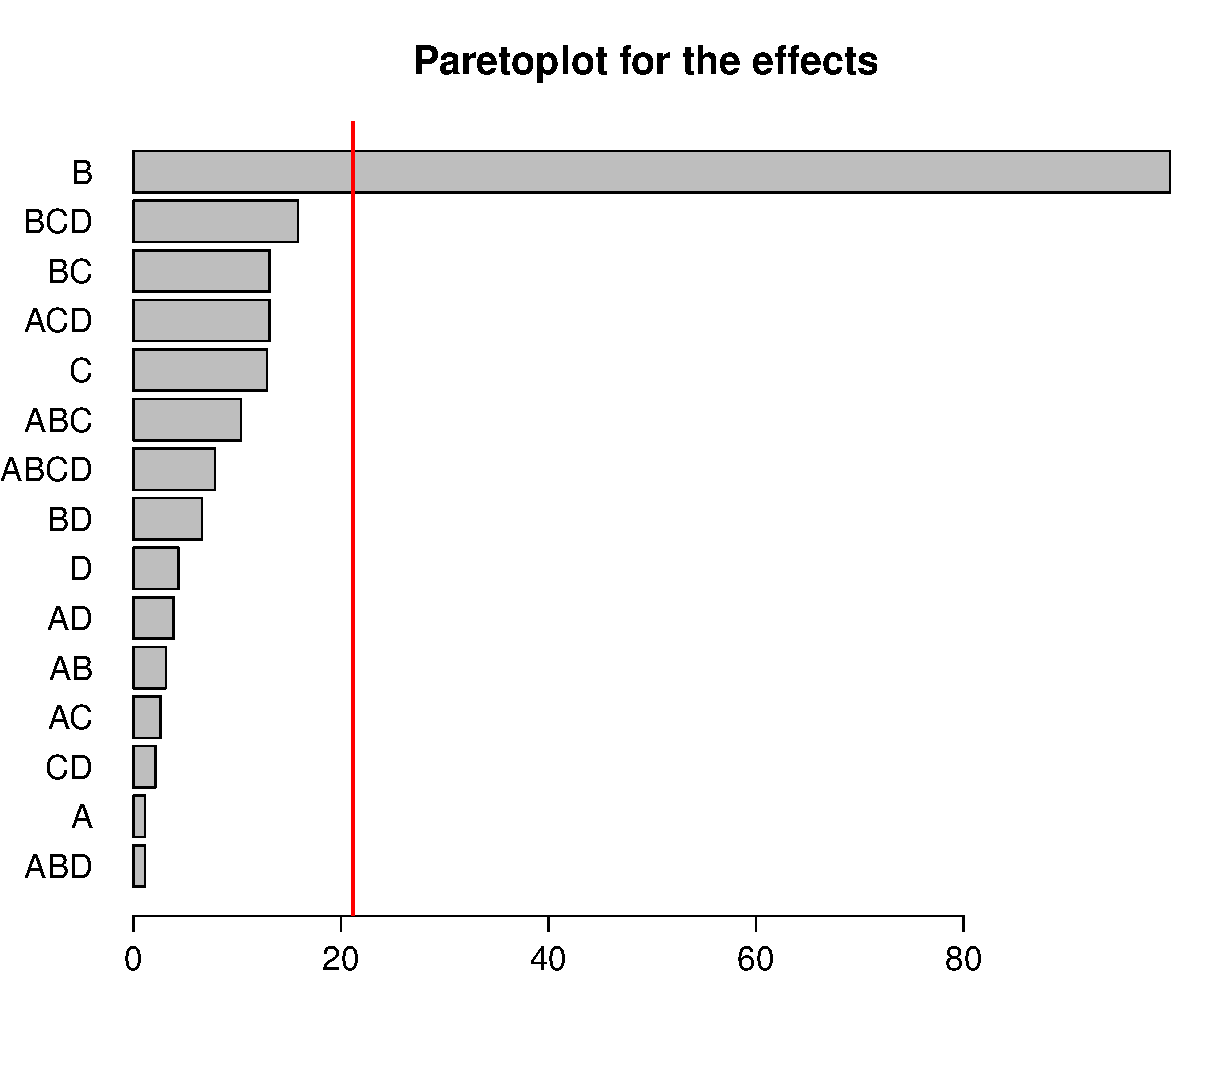
\includegraphics[width=0.6\textwidth]{PDF/paretoPlot.pdf}
    \caption{Awesome Image}
    \label{fig:awesome_image}
\end{figure}

\begin{figure}[p]
    \centering
    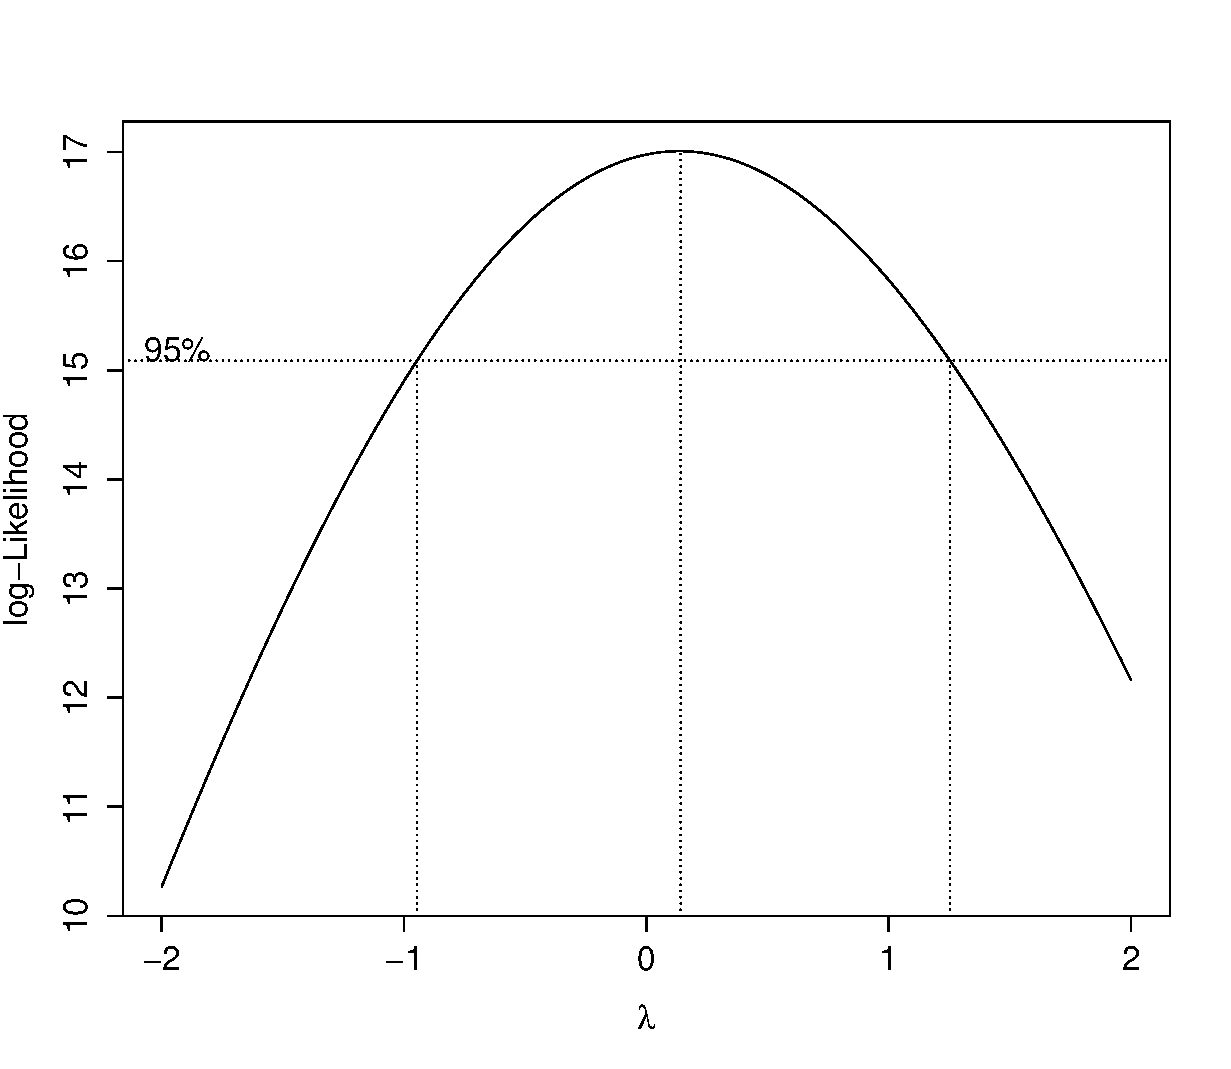
\includegraphics[width=0.6\textwidth]{PDF/boxCox.pdf}
    \caption{Awesome Image}
    \label{fig:awesome_image}
\end{figure}

\begin{figure}[p]
    \centering
    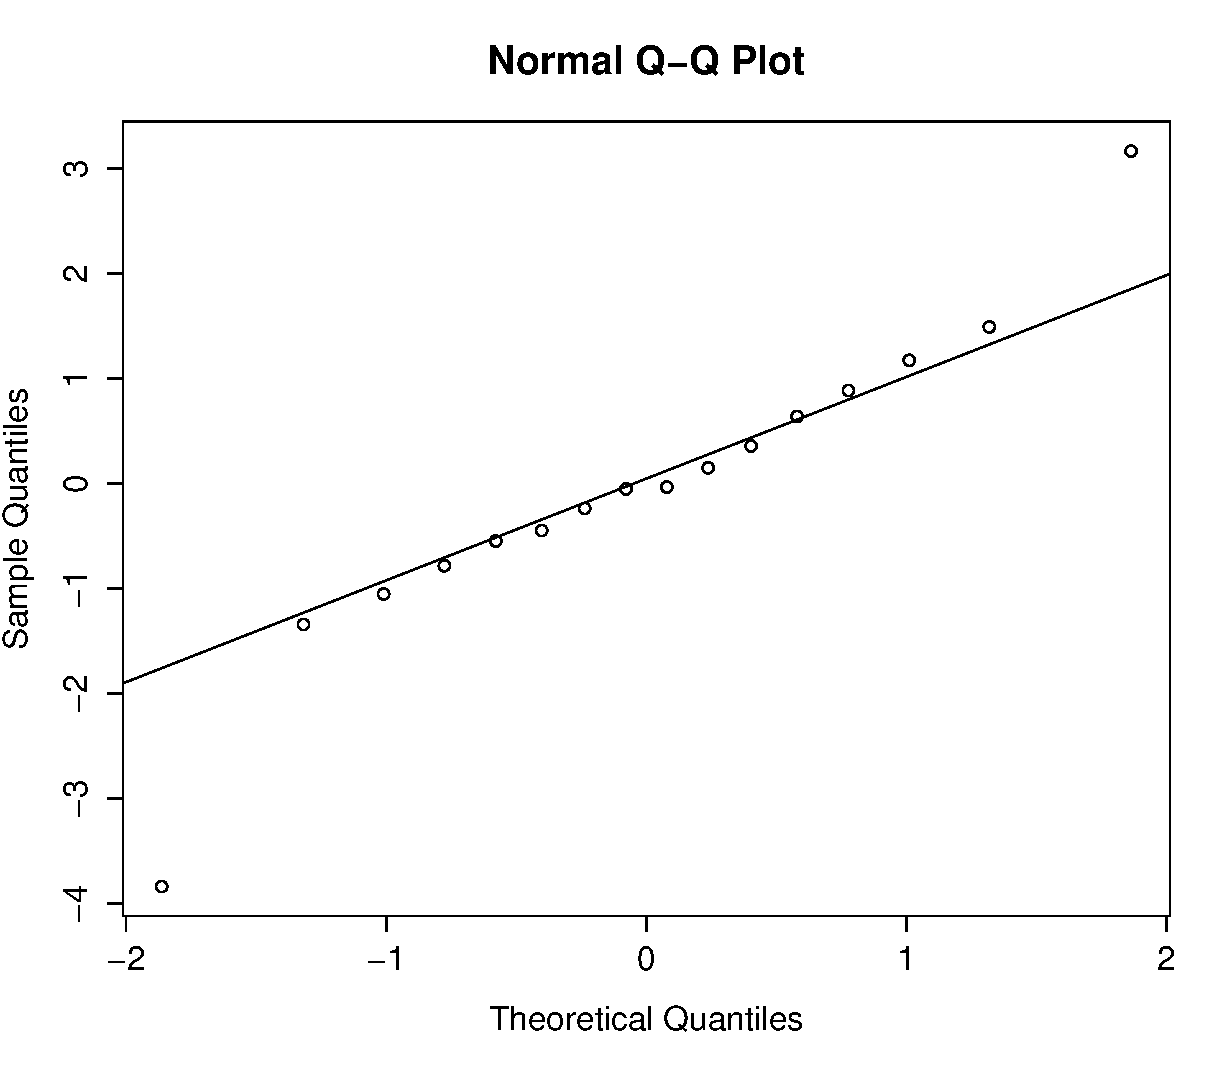
\includegraphics[width=0.6\textwidth]{PDF/qqPlot.pdf}
    \caption{Awesome Image}
    \label{fig:awesome_image}
\end{figure}

\begin{figure}[p]
    \centering
    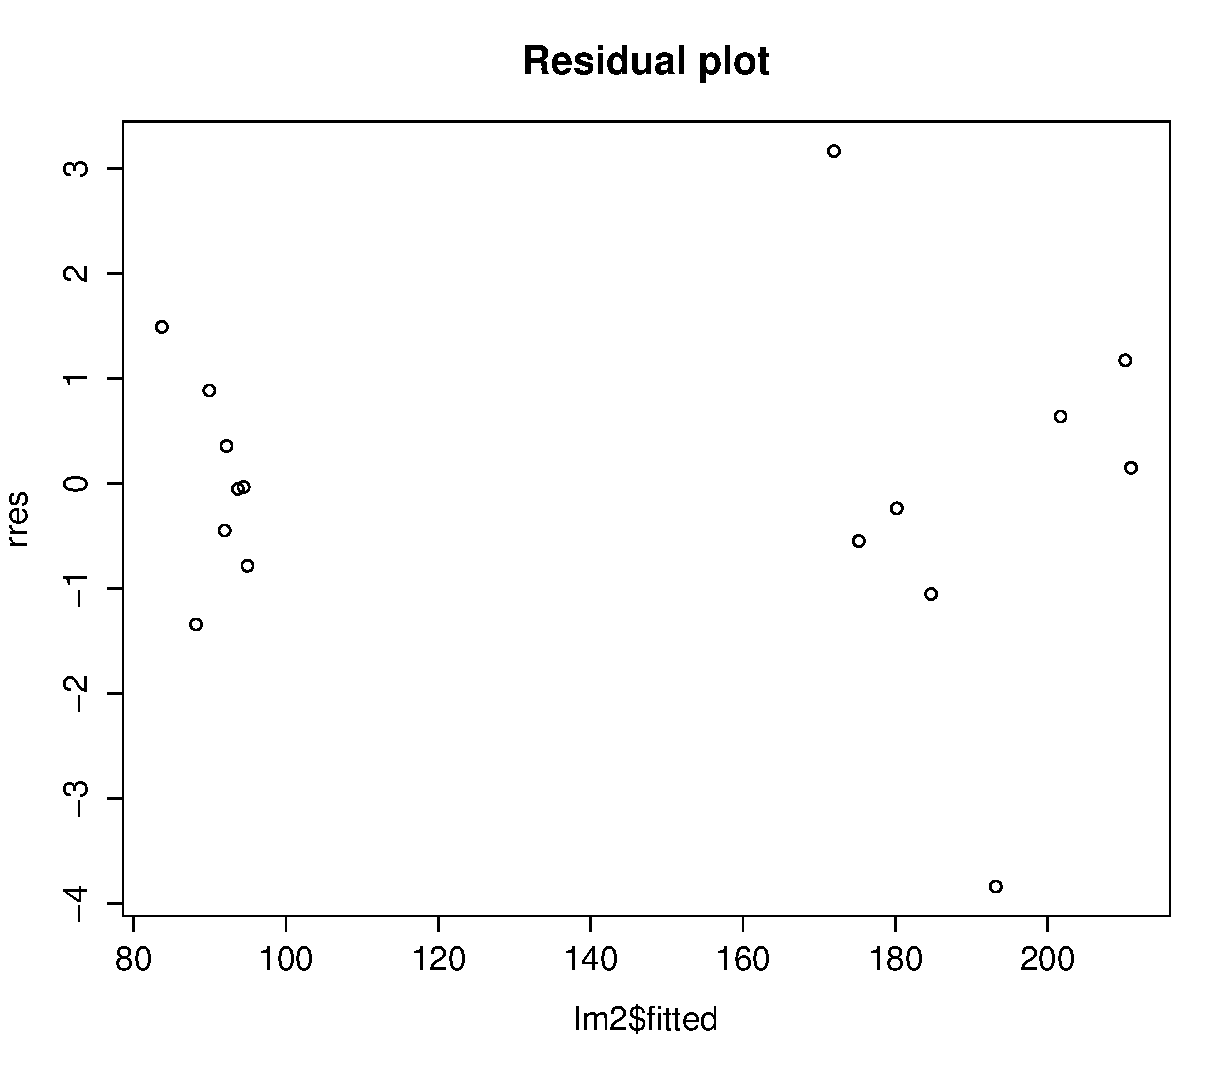
\includegraphics[width=0.6\textwidth]{PDF/residualPlot.pdf}
    \caption{Awesome Image}
    \label{fig:awesome_image}
\end{figure}

\begin{figure}[p]
    \centering
    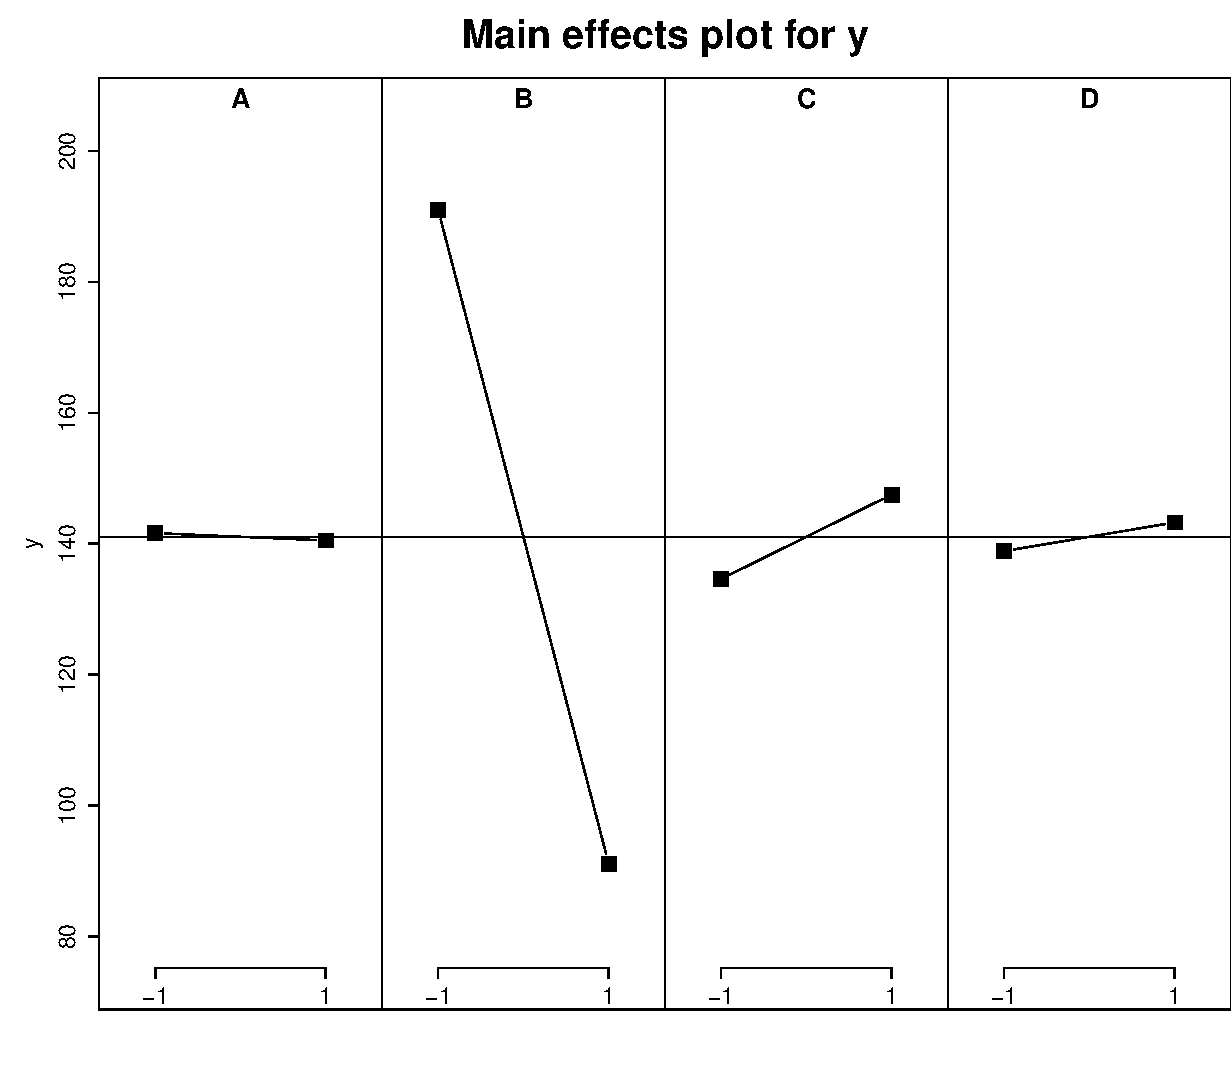
\includegraphics[width=0.6\textwidth]{PDF/mainEffects4factors.pdf}
    \caption{Awesome Image}
    \label{fig:awesome_image}
\end{figure}

\begin{figure}[p]
    \centering
    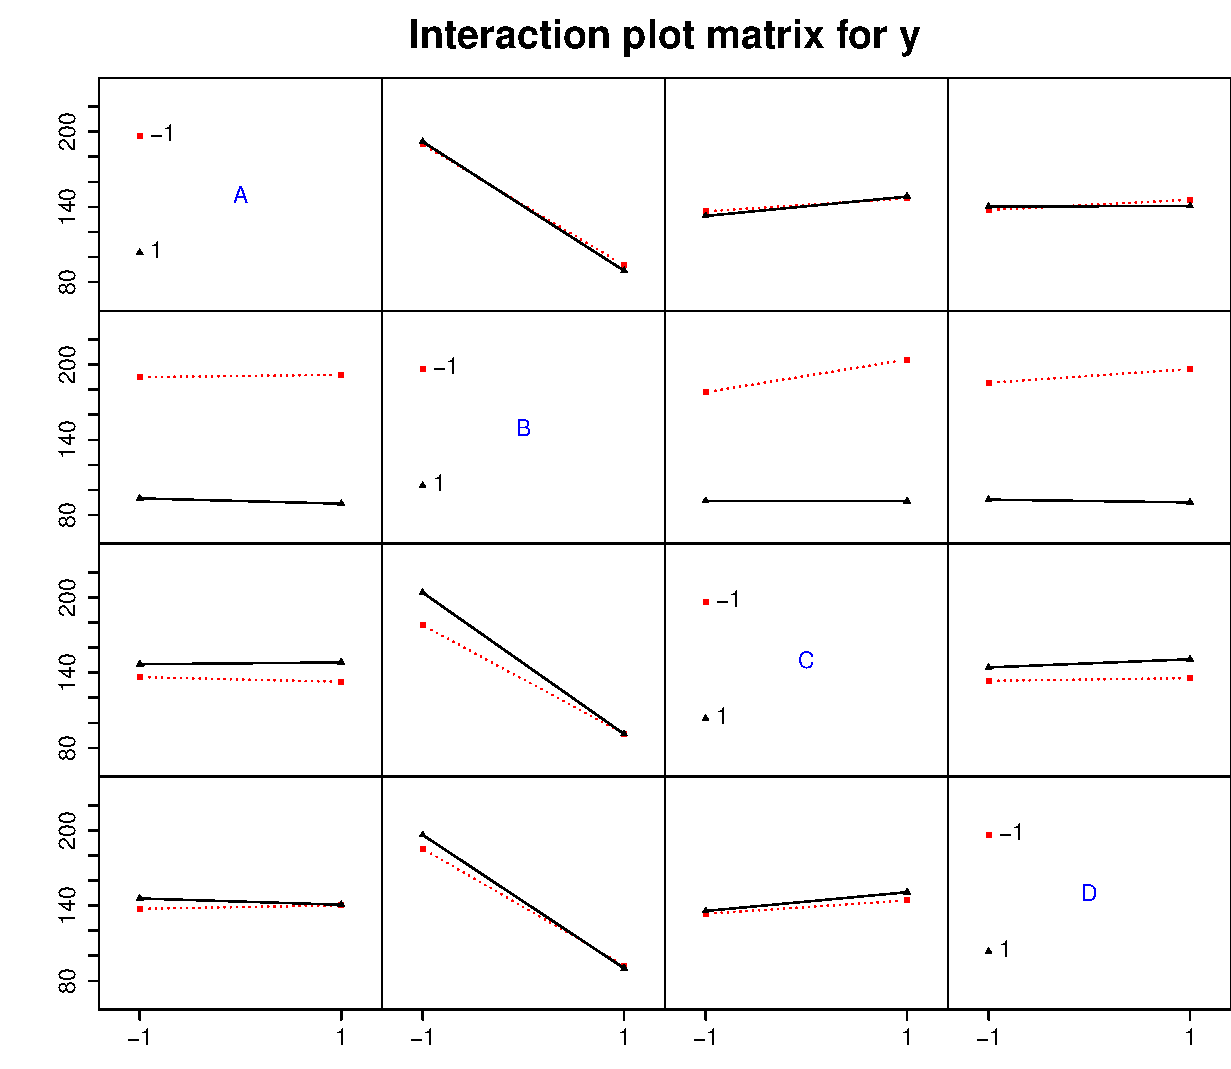
\includegraphics[width=0.6\textwidth]{PDF/interactionPlot4factors.pdf}
    \caption{Awesome Image}
    \label{fig:awesome_image}
\end{figure}


\section{Conclusions and recommendations}
a

\newpage

\begin{thebibliography}{9}
\bibitem{teaTemperatures}
  \emph{Tea Tips: Water Temperature}.
  http://www.twoleavestea.com/water-temperature, 04/04-2014
\end{thebibliography}

\end{document}